\chapter{Lập trình hợp ngữ Assembly}

\section{Bài tập của Nguyễn Trường Thái}

\subsection{Chuyển ký tự thường thành ký tự hoa}
Chương trình hợp ngữ Assembly cho phép nhập 1 ký tự viết thường và in ra màn hình chữ hoa của ký tự đó.

\begin{figure}[H]
    \centering
     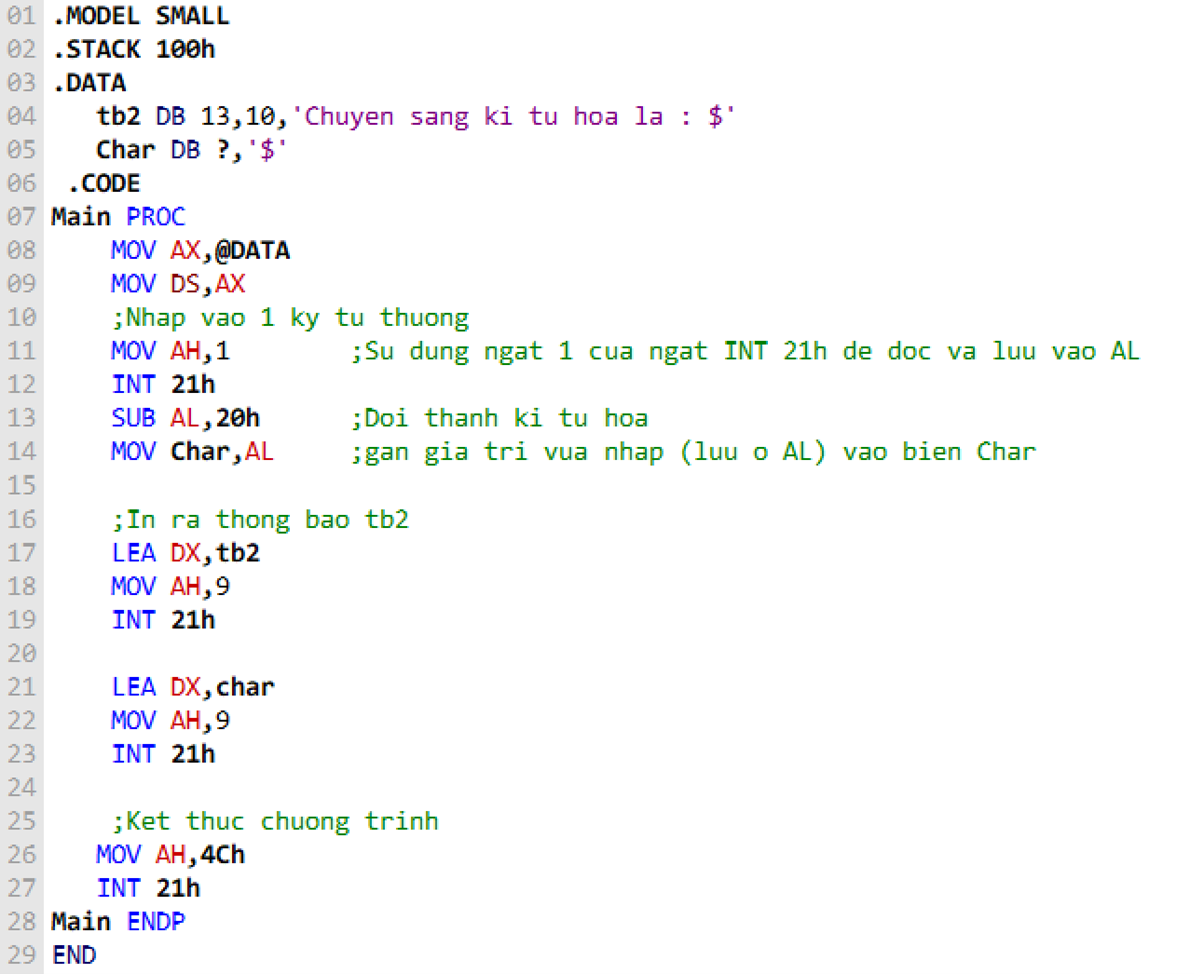
\includegraphics[width=0.9\textwidth]{Thái/Picture1.png}
    \caption{Mã nguồn in ra ký tự theo dạng viết hoa}
\end{figure}


\begin{figure}[H]
    \centering
     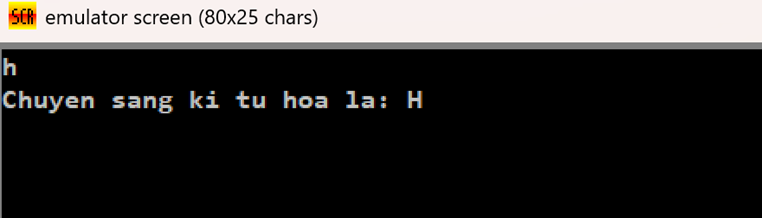
\includegraphics[width=0.8\textwidth]{Thái/Picture2.png}
    \caption{Giao diện in ra ký tự theo dạng viết hoa}
\end{figure}

\subsection{Chuyển số từ hệ cơ số 10 sang hệ cơ số 16}
Chương trình hợp ngữ Assembly chuyển một số từ hệ cơ số 10 sang hệ cơ số 16 (Hexa).

\begin{figure}[H]
    \centering
    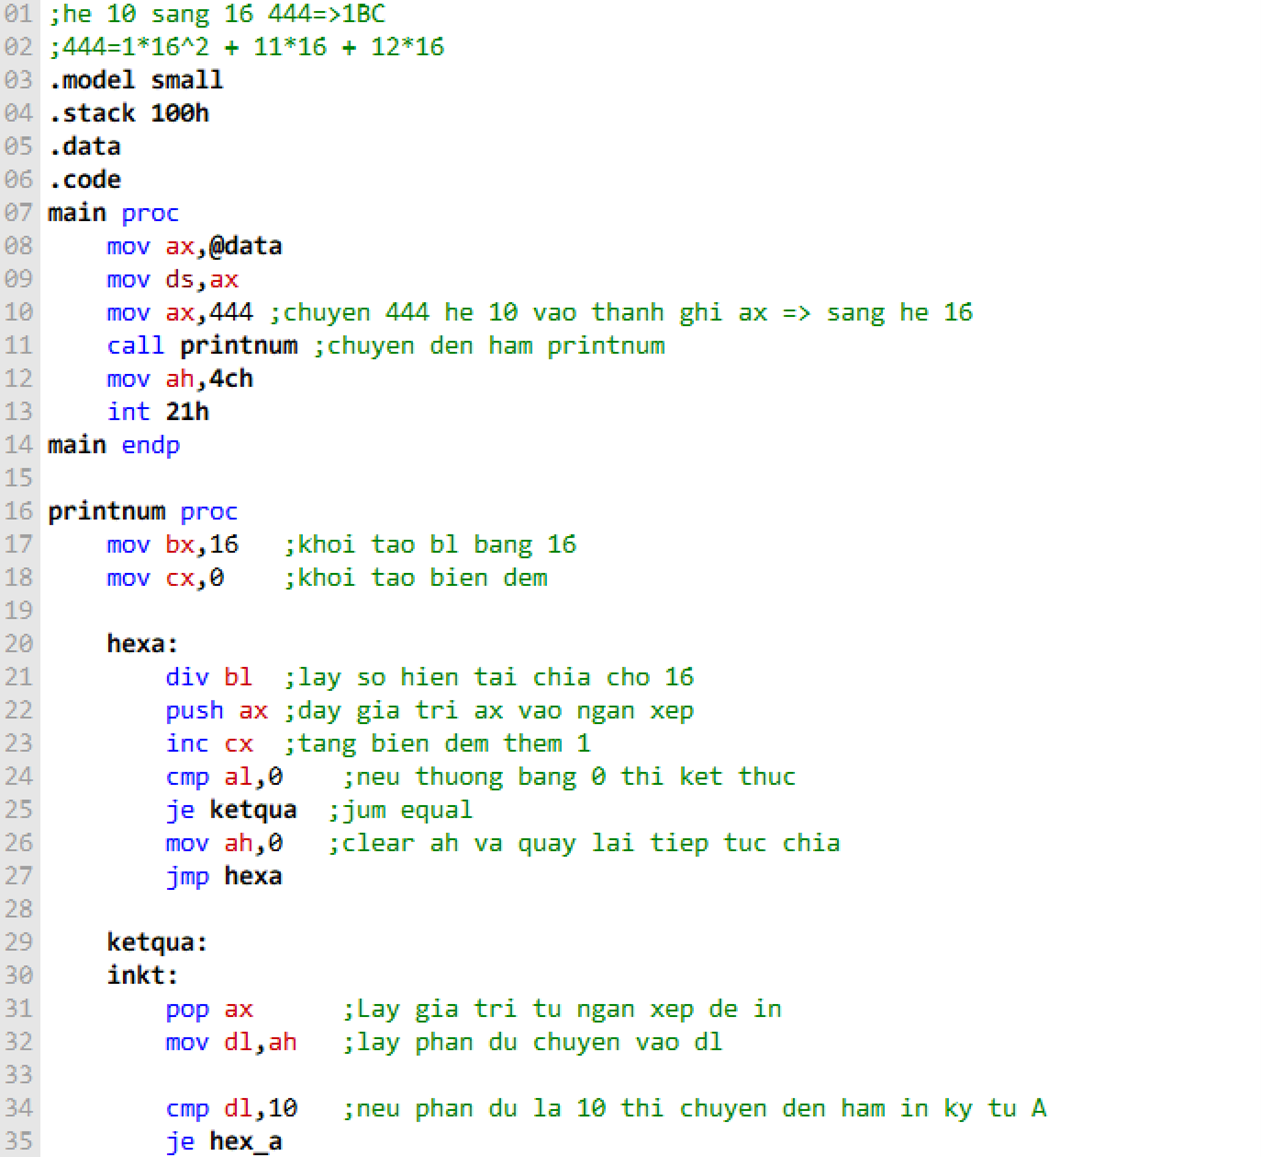
\includegraphics[width=0.9\textwidth]{Thái/Picture3.png}
\end{figure}

\begin{figure}[H]
    \centering
    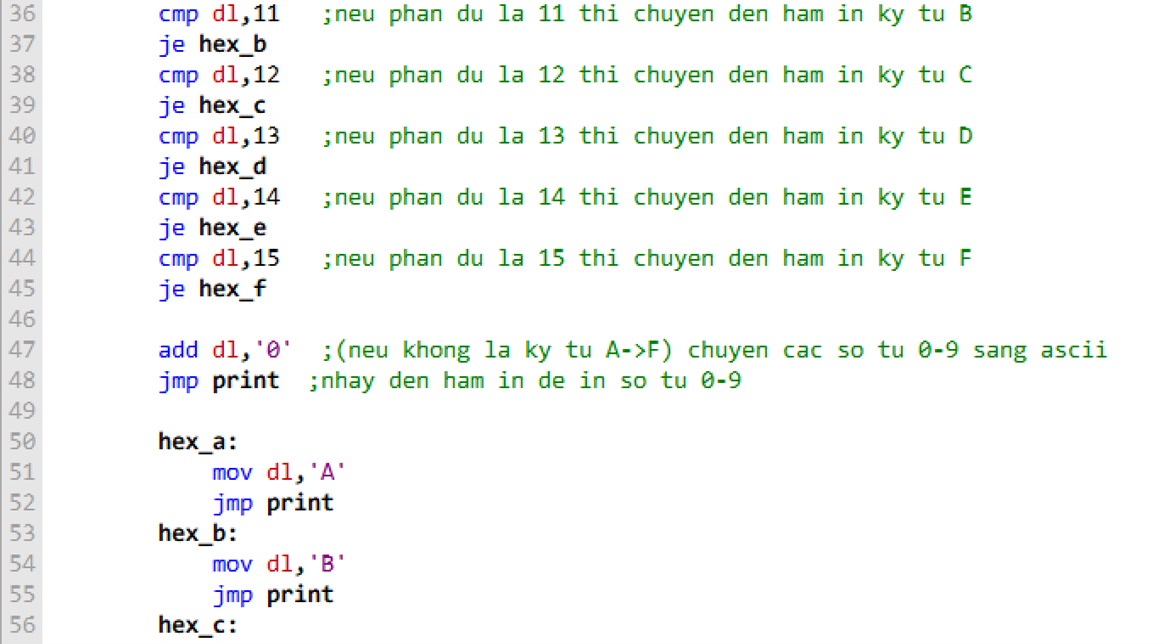
\includegraphics[width=0.9\textwidth]{Thái/Picture4.png}
     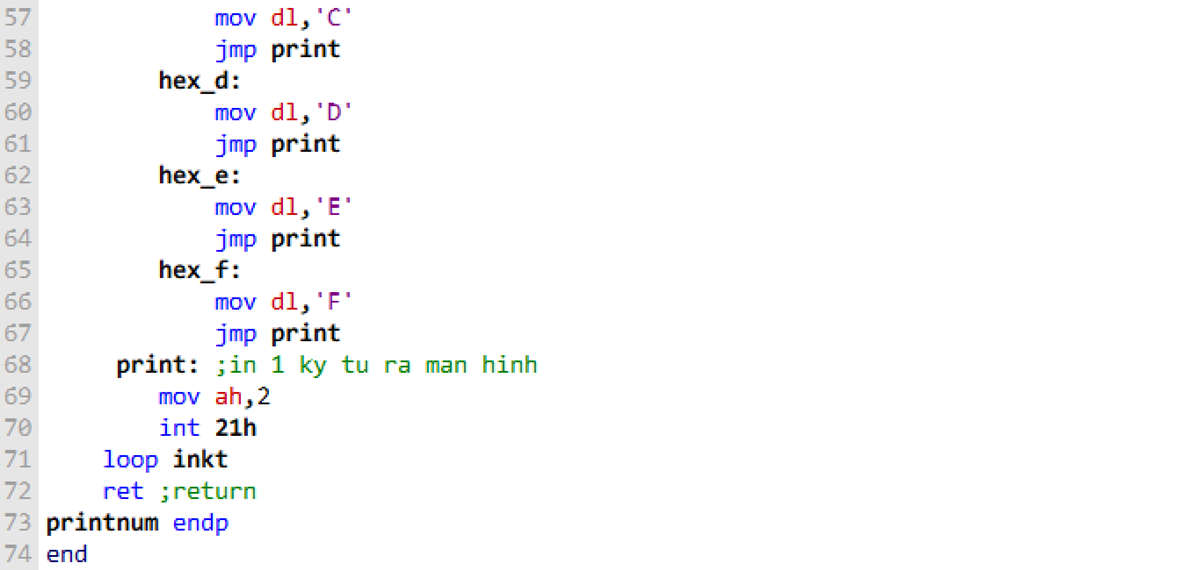
\includegraphics[width=0.9\textwidth]{Thái/Picture5.png}
    \caption{Mã nguồn in ra chuyển số 444 từ hệ cơ số 10 sang hệ cơ số 16}
\end{figure}


\begin{figure}[H]
    \centering
      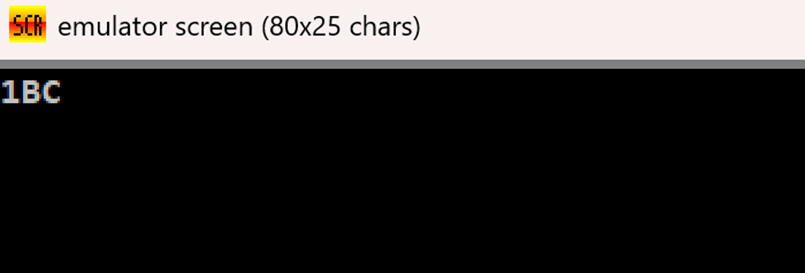
\includegraphics[width=0.9\textwidth]{Thái/Picture6.png}
    \caption{Giao diện in ra giá trị 444 từ hệ cơ số 10 sang hệ cơ số 16}
\end{figure}

\subsection{Tính tổng 2 số kiểu word}
Chương trình hợp ngữ Assembly tính tổng 2 số kiểu word.

\begin{figure}[H]
    \centering
    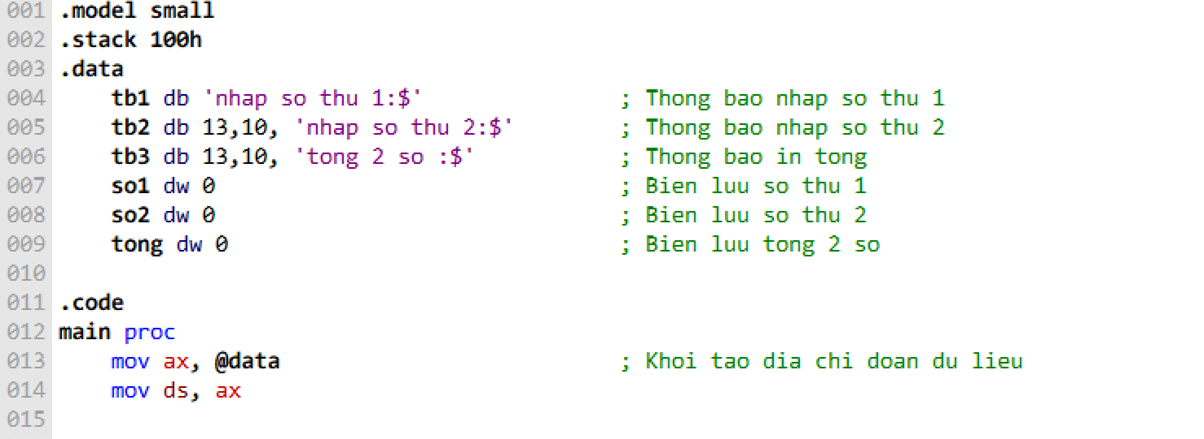
\includegraphics[width=0.9\textwidth]{Thái/Picture7.png}
      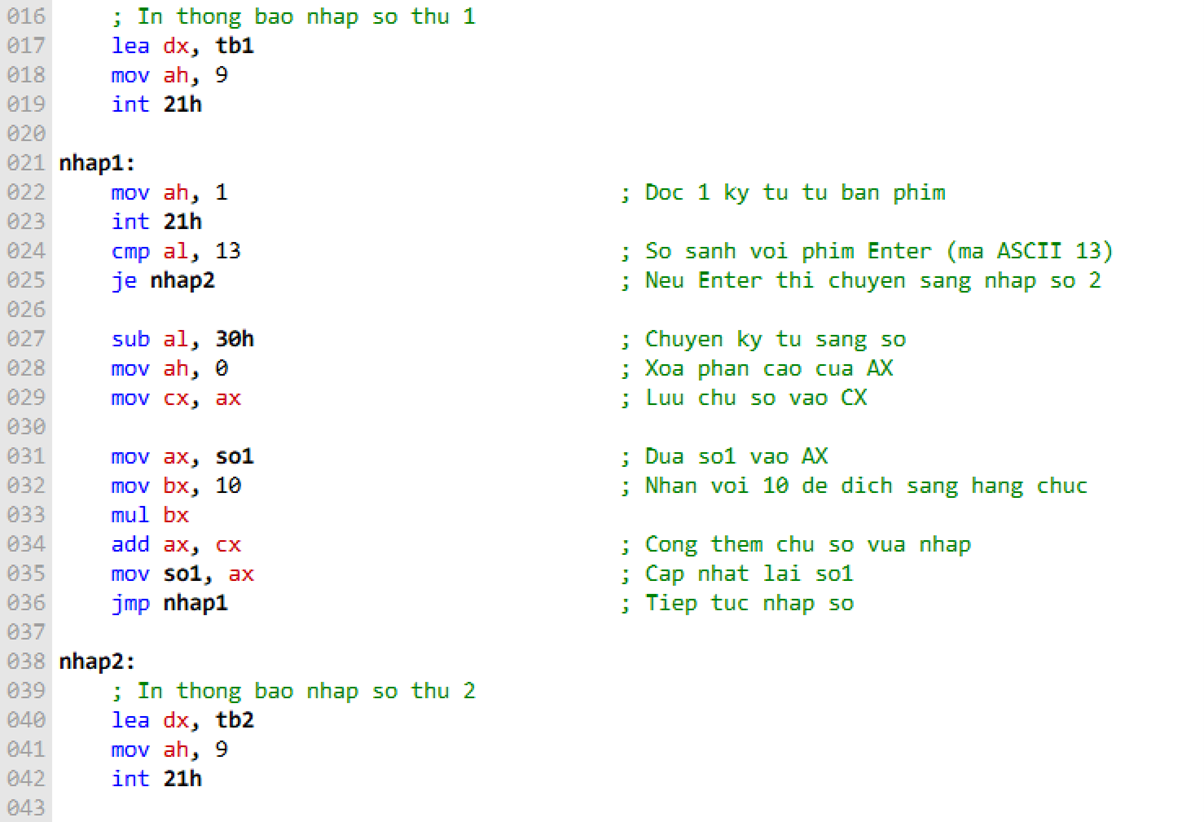
\includegraphics[width=0.9\textwidth]{Thái/Picture8.png}
\end{figure}


\begin{figure}[H]
    \centering
    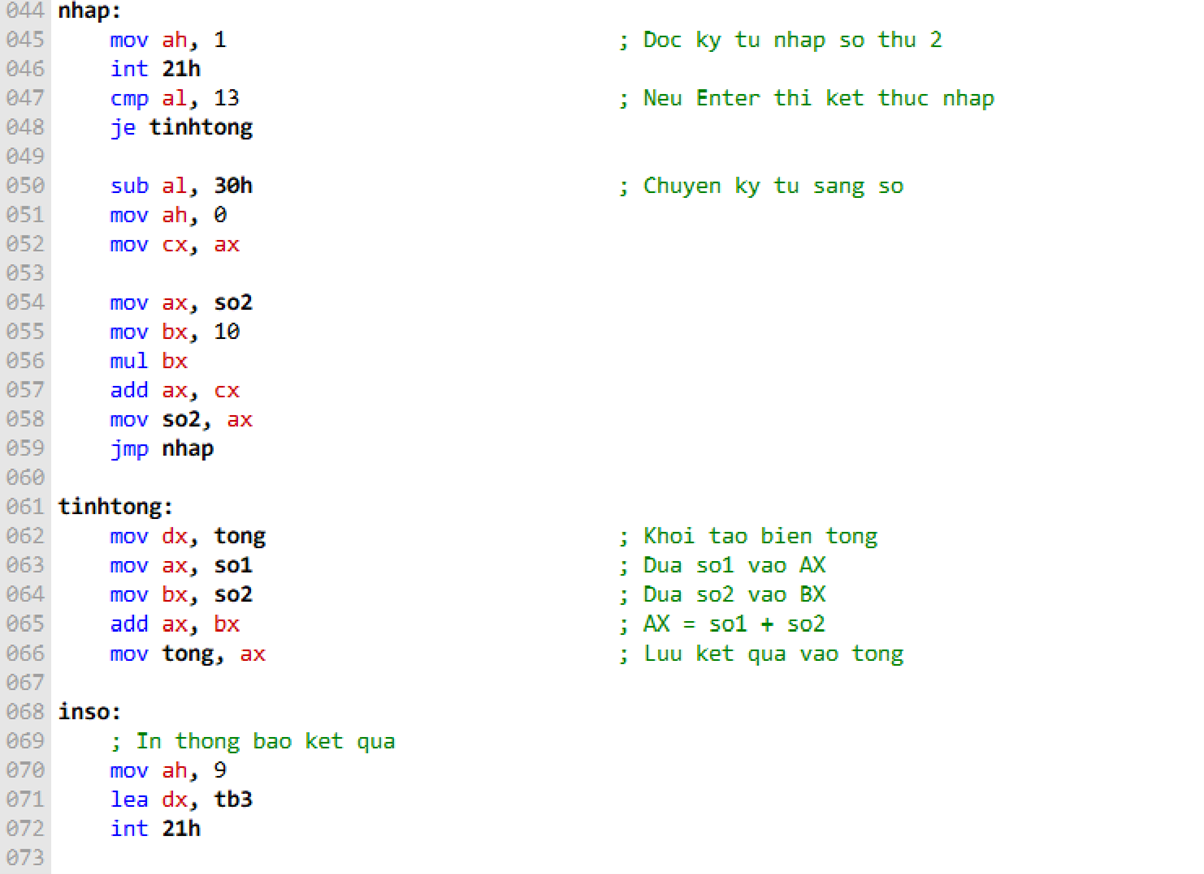
\includegraphics[width=0.9\textwidth]{Thái/Picture9.png}
     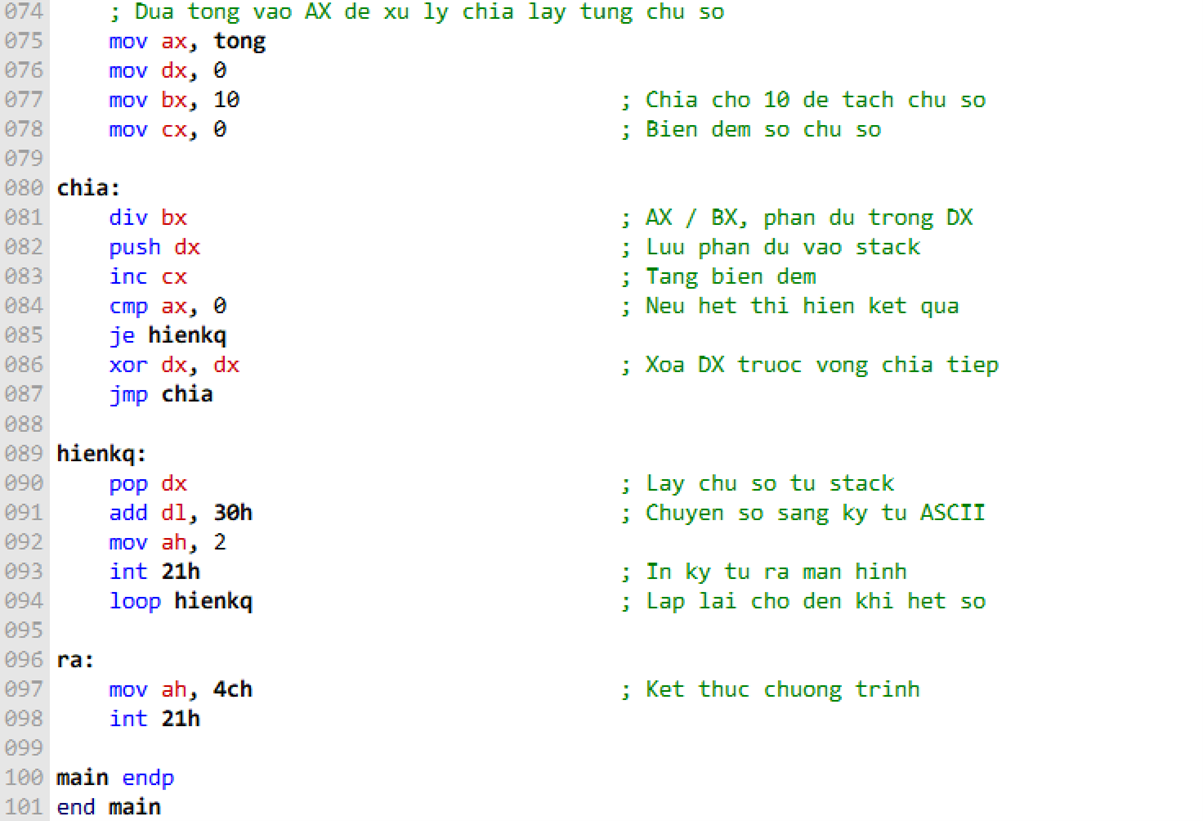
\includegraphics[width=0.9\textwidth]{Thái/Picture10.png}
    \caption{Mã nguồn in ra tổng 2 số theo kiểu word}
\end{figure}

\begin{figure}[H]
    \centering
      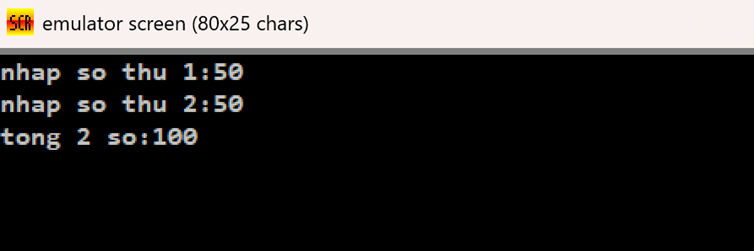
\includegraphics[width=0.9\textwidth]{Thái/Picture11.png}
    \caption{Giao diện in ra tổng 2 số theo kiểu word}
\end{figure}

\section{Bài tập của Vũ Quang Huy}

\subsection{Chuyển chuỗi ký tự thành dạng viết hoa và viết thường}
Chương trình hợp ngữ Assembly cho phép nhập 1 chuỗi ký tự, in ra màn hình chuỗi ký tự đó theo dạng viết hoa và viết thường.

\begin{figure}[H]
    \centering
    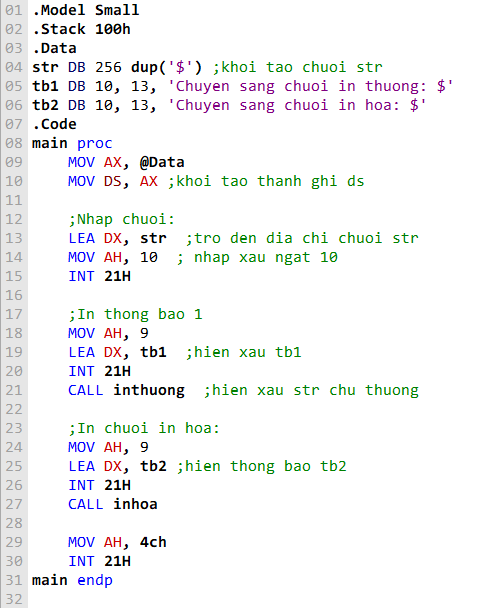
\includegraphics[width=0.8\textwidth]{Huy/1.5.1.png}
\end{figure}

\begin{figure}[H]
    \centering
    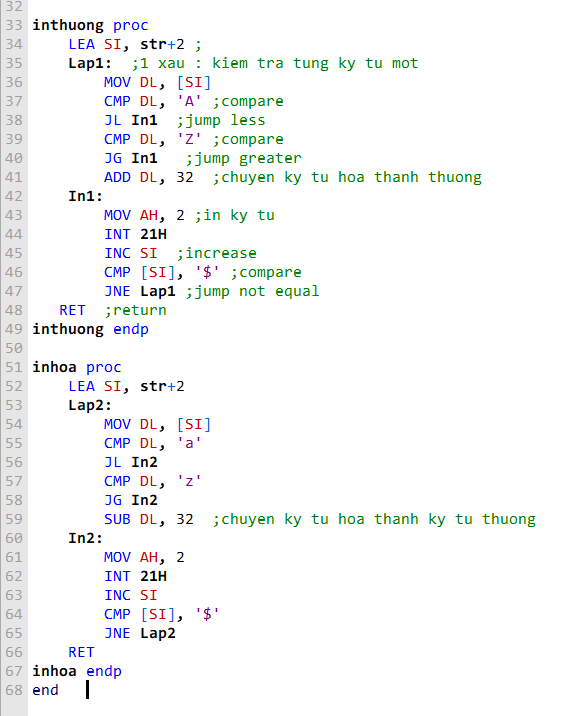
\includegraphics[width=0.8\textwidth]{Huy/1.5.2.png}
    \caption{Mã nguồn in ra chuỗi theo dạng viết hoa và viết thường}
\end{figure}

\begin{figure}[H]
    \centering
    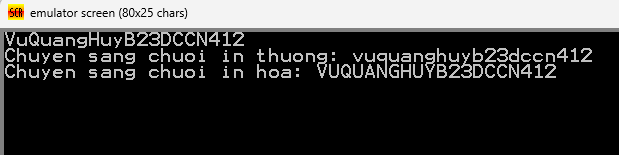
\includegraphics[width=0.8\textwidth]{Huy/1.5.3.png}
    \caption{Giao diện in ra chuỗi theo dạng viết hoa và viết thường}
\end{figure}

\subsection{In chuỗi ký tự theo thứ tự ngược lại}
Chương trình hợp ngữ Assembly cho phép nhập một chuỗi các ký tự kết thúc bởi ``\#'' và yêu cầu in ra màn hình chuỗi ký tự đó theo thứ tự ngược lại.

\begin{figure}[H]
    \centering
    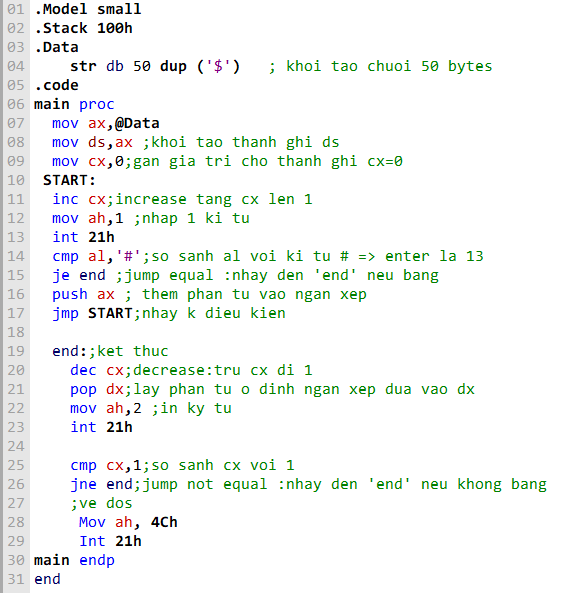
\includegraphics[width=0.8\textwidth]{Huy/1.6.1.png}
    \caption{Mã nguồn in ra chuỗi kết thúc bởi '\#' theo thứ tự ngược lại}
\end{figure}

\begin{figure}[H]
    \centering
     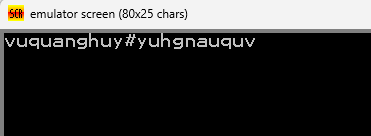
\includegraphics[width=0.8\textwidth]{Huy/1.6.2.png}
    \caption{Giao diện in ra chuỗi kết thúc bởi '\#' theo thứ tự ngược lại}
\end{figure}

\subsection{Tìm giá trị lớn nhất và nhỏ nhất của một mảng số}
Chương trình hợp ngữ Assembly tìm giá trị lớn nhất và nhỏ nhất của một mảng số.

\begin{figure}[H]
    \centering
     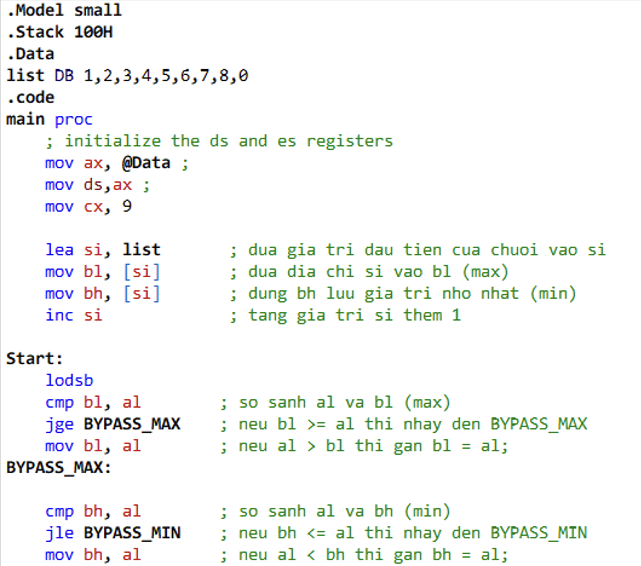
\includegraphics[width=0.8\textwidth]{Huy/1.11.1.png}
\end{figure}

\begin{figure}[H]
    \centering
     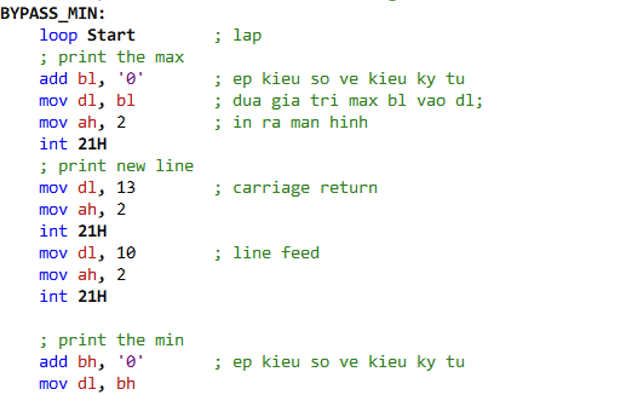
\includegraphics[width=0.8\textwidth]{Huy/1.11.2.png}
    \caption{Mã nguồn in ra giá trị lớn nhất và nhỏ nhất của mảng số}
\end{figure}

\begin{figure}[H]
    \centering
      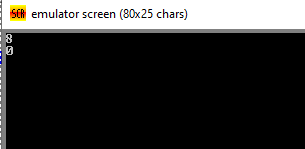
\includegraphics[width=0.8\textwidth]{Huy/1.11.3.png}
    \caption{Giao diện in ra giá trị lớn nhất và nhỏ nhất của mảng số}
\end{figure}

\section{Bài tập của Lê Huy Hải}

\subsection{Chuyển số từ hệ cơ số 10 sang hệ nhị phân}
Chương trình hợp ngữ Assembly chuyển một số từ hệ cơ số 10 sang hệ nhị phân.

\begin{figure}[H]
    \centering
    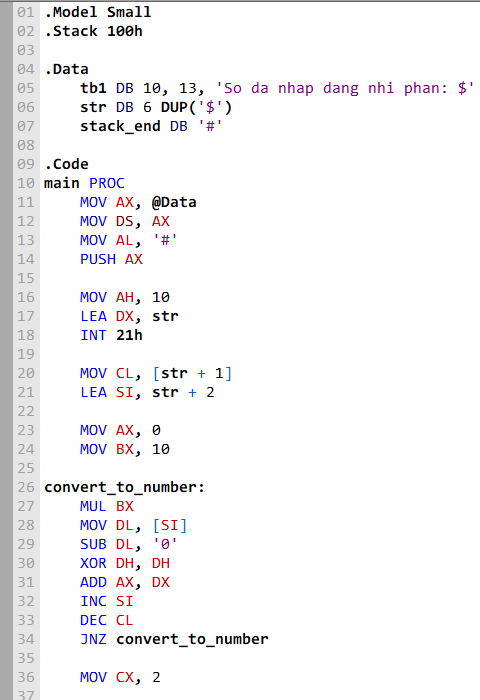
\includegraphics[width=0.8\textwidth]{Hải/Image_01.png}
\end{figure}

\begin{figure}[H]
    \centering
    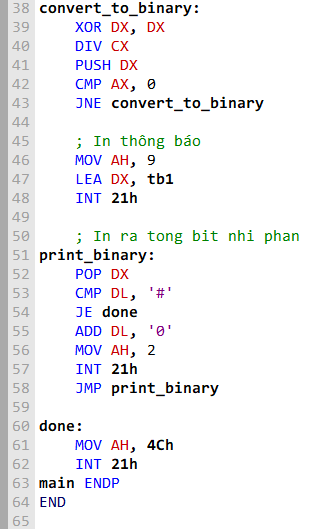
\includegraphics[width=0.8\textwidth]{Hải/Image_02.png}
    \caption{Mã nguồn chuyển số từ hệ cơ số 10 sang hệ nhị phân}
\end{figure}

\begin{figure}[H]
    \centering
     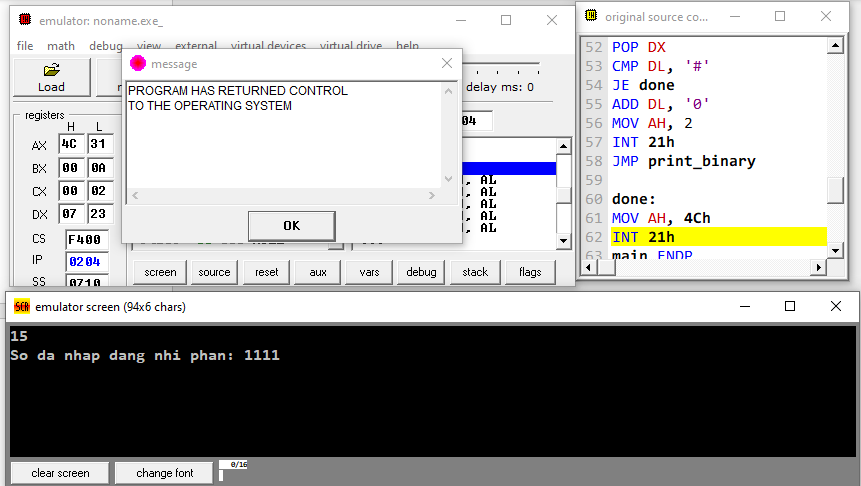
\includegraphics[width=0.8\textwidth]{Hải/Image_03.png}
    \caption{Kết quả in ra khi đã chuyển đổi sang hệ nhị phân}
\end{figure}

\subsection{Đếm chiều dài của một chuỗi ký tự}
Chương trình hợp ngữ Assembly yêu cầu đếm chiều dài của một chuỗi ký tự cho trước.

\begin{figure}[H]
    \centering
     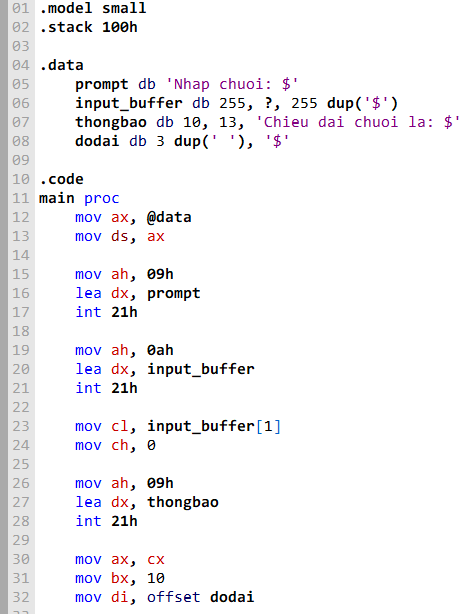
\includegraphics[width=0.8\textwidth]{Hải/Image_04.png}
\end{figure}


\begin{figure}[H]
    \centering
     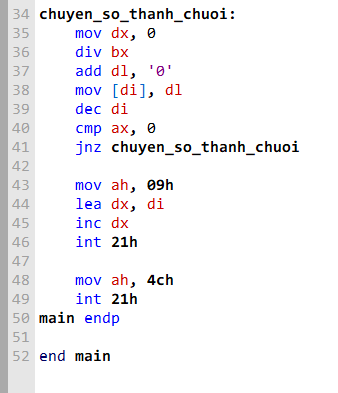
\includegraphics[width=0.8\textwidth]{Hải/Image_05.png}
    \caption{Mã Nguồn đếm chiều dài của xâu kí tự cho trước}
\end{figure}

\begin{figure}[H]
    \centering
     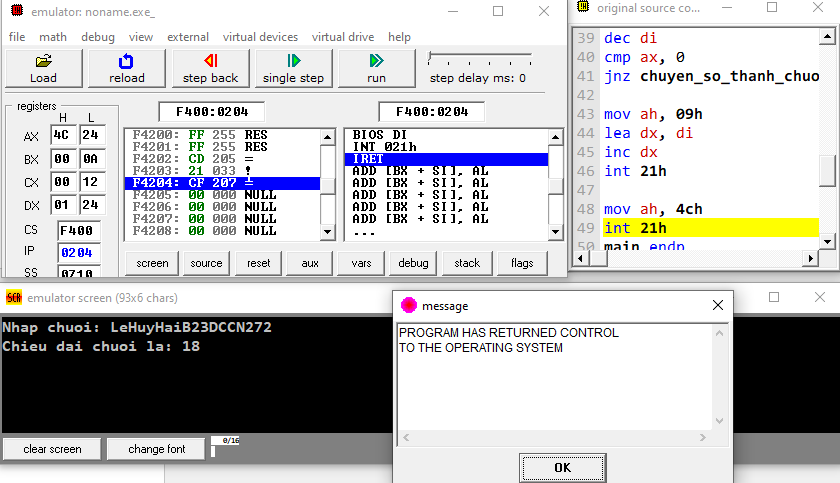
\includegraphics[width=0.8\textwidth]{Hải/Image_06.png}
    \caption{Kết quả in ra khi tính chiều dài của chuỗi}
\end{figure}

\subsection{Tính tổng các số}
Chương trình hợp ngữ Assembly cho phép nhập vào các số và in ra màn hình tổng của các số đó.

\begin{figure}[H]
    \centering
     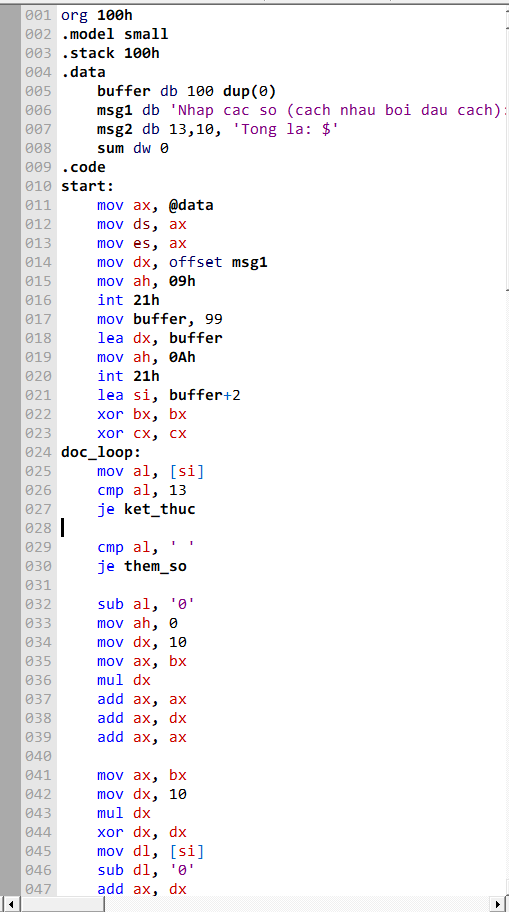
\includegraphics[width=0.7\textwidth]{Hải/Image_07.png}
\end{figure}

\begin{figure}[H]
    \centering
     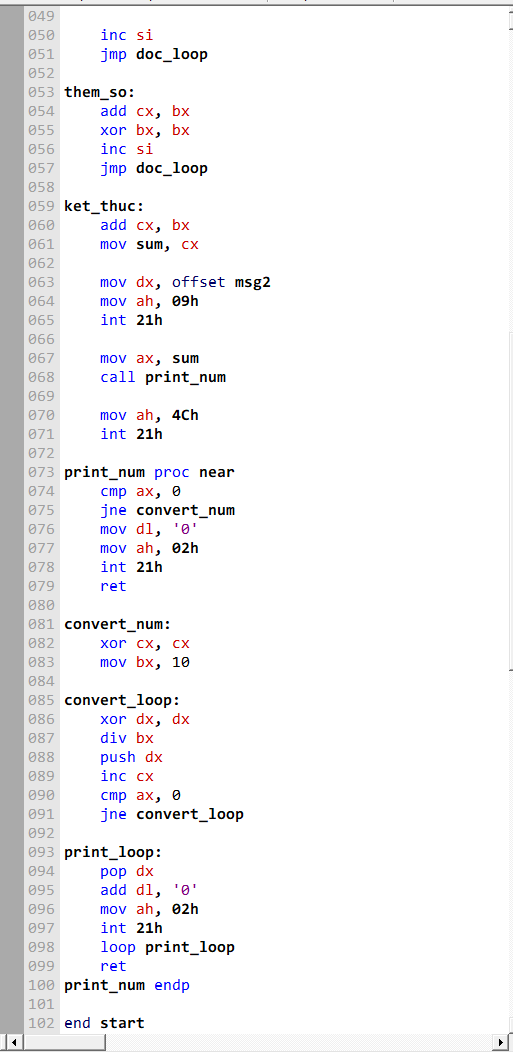
\includegraphics[width=0.7\textwidth]{Hải/Image_08.png}
    \caption{Mã nguồn in ra tổng các số cho trước}
\end{figure}

\begin{figure}[H]
    \centering
     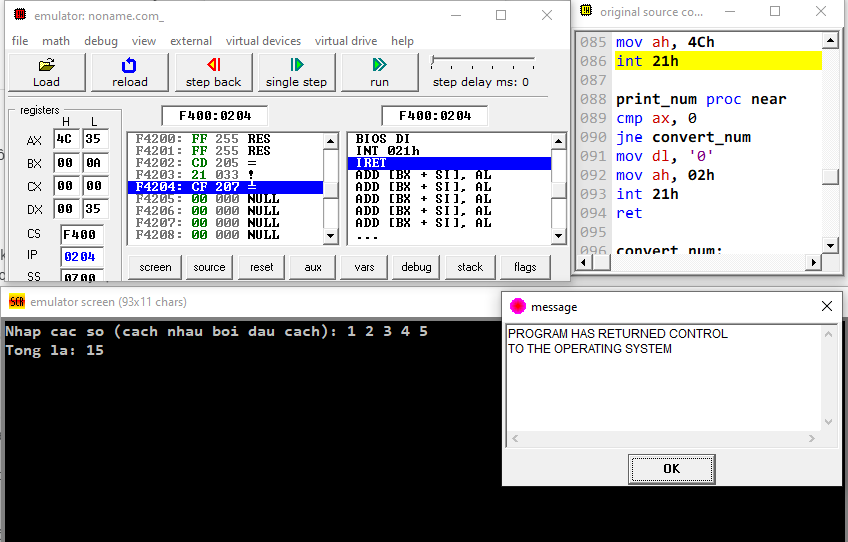
\includegraphics[width=0.8\textwidth]{Hải/Image_09.png}
    \caption{Kết quả in ra tổng của các số đã cho}
\end{figure}

\section{Bài tập của Hà Duy Khánh}

\subsection{Lời chào tiếng Anh \& tiếng Việt}
Chương trình hợp ngữ Assembly hiển thị lời chào bằng tiếng Anh và tiếng Việt.

\begin{figure}[H]
    \centering
     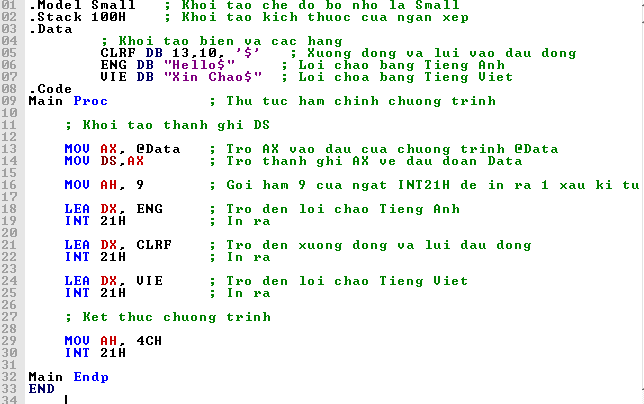
\includegraphics[width=0.8\textwidth]{Khánh/1.png}    
    \caption{Mã nguồn in ra lời chào bằng tiếng Việt và tiếng Anh}
\end{figure}

\begin{figure}[H]
    \centering
     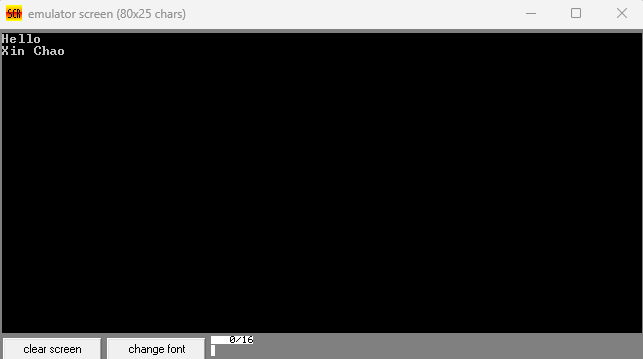
\includegraphics[width=0.8\textwidth]{Khánh/2.png}
    \caption{Kết quả in ra lời chào bằng tiếng Việt và tiếng Anh}
\end{figure}

\subsection{Nhập 1 ký tự và in ra}
Chương trình hợp ngữ Assembly nhập một ký tự và hiển thị ra màn hình.

\begin{figure}[H]
    \centering
     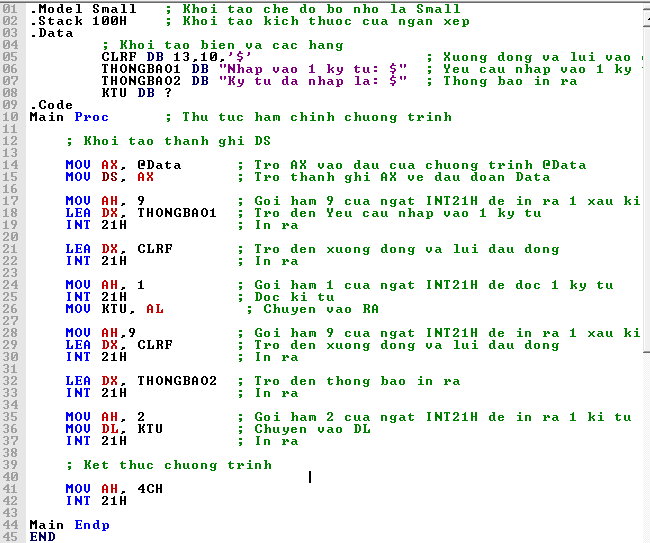
\includegraphics[width=0.8\textwidth]{Khánh/3.png}
    \caption{Mã nguồn nhập 1 ký tự và hiện thị ra màn hình}
\end{figure}

\begin{figure}[H]
    \centering
     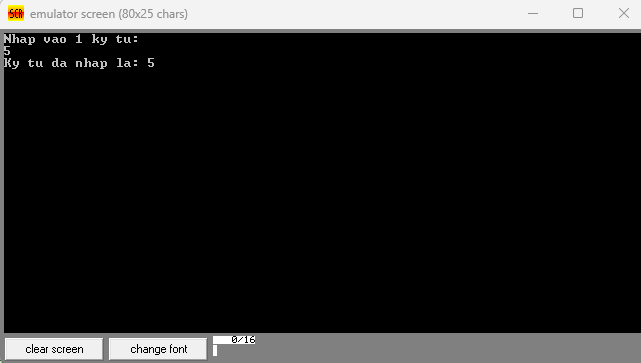
\includegraphics[width=0.8\textwidth]{Khánh/4.png}
    \caption{Giao diện hiện thị 1 ký tự ra màn hình}
\end{figure}

\subsection{Tính giai thừa}
Chương trình hợp ngữ Assembly tính giai thừa của một số.

\begin{figure}[H]
    \centering
     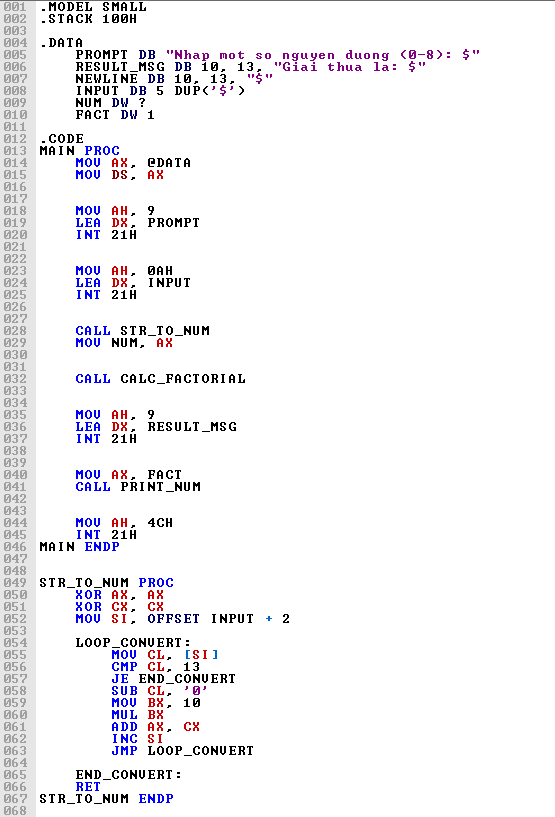
\includegraphics[width=0.8\textwidth]{Khánh/5.png}
\end{figure}
\begin{figure}[H]
    \centering
     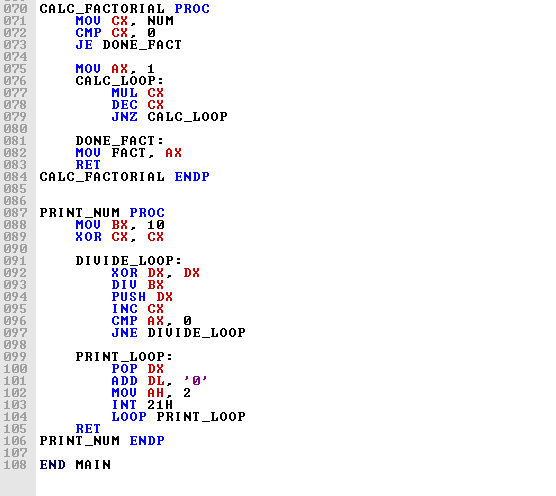
\includegraphics[width=0.8\textwidth]{Khánh/6.png}
    \caption{Mã nguồn tính giai thừa của 1 số}
\end{figure}
\begin{figure}[H]
    \centering
     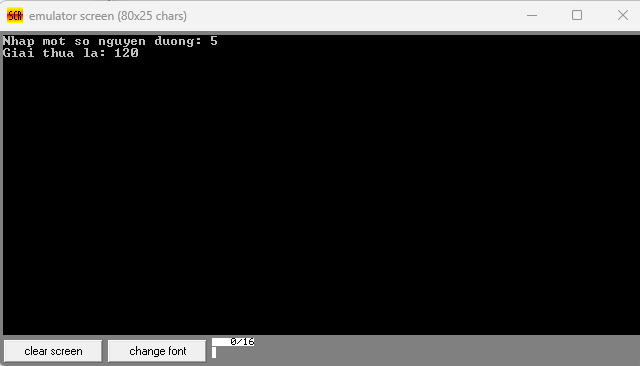
\includegraphics[width=0.8\textwidth]{Khánh/7.png}
    \caption{Kết quả phép tính giai thừa của 1 số}
\end{figure}
